\chapter{The Delay Experiment}\label{ch:Implementation}

\section{A3.1 -- Where Does the Time Go?}
Each of T1--T5 was pinged 50 times; Table~\ref{tab:rttstats} records the minimum, average, and
maximum RTT observed for each. Distances are rough straight-line estimates -- T2/T4 from map
distance to the named campus, T3/T5 from public IP geolocation (the resolved IP's registered
location) -- and are not independently verified against ground truth.

\begin{table}[H]
\centering
\caption{Aggregate RTT statistics, 50 packets per target.}
\label{tab:rttstats}
\footnotesize
\begin{tabular}{@{}p{2.6cm}p{2.6cm}cccc@{}}
\toprule
Target (role) & Resolved IP & Est. distance & Min RTT & Avg RTT & Max RTT \\
\midrule
T1 (local gateway) & 10.184.0.13 & $<$0.1 km & 3.904 & 8.891 & 96.290 \\
T2 (campus target) & www.iitd.ac.in & $\sim$2.0 km & 3.315 & 7.489 & 14.110 \\
T3 (regional DNS) & 8.8.8.8 & $\sim$20.0 km & 42.824 & 49.859 & 119.830 \\
T4 (IIT Bombay) & www.iitb.ac.in & $\sim$1100 km & \multicolumn{3}{c}{N/A -- 100\% packet loss} \\
T5 (global target) & www.mit.edu & nominal 12{,}000 km & 35.596 & 51.145 & 247.982 \\
\bottomrule
\end{tabular}

{\footnotesize All RTT values in ms.}
\end{table}

T4 returned 100\% packet loss across all 50 probes. We read this as ICMP being firewalled at or
near \texttt{www.iitb.ac.in} rather than a routing failure -- traceroutes toward the same
destination (Chapter~\ref{ch:Design}) do get responses from intermediate hops, which would not
happen if the path itself were broken.

\begin{figure}[H]
    \centering
    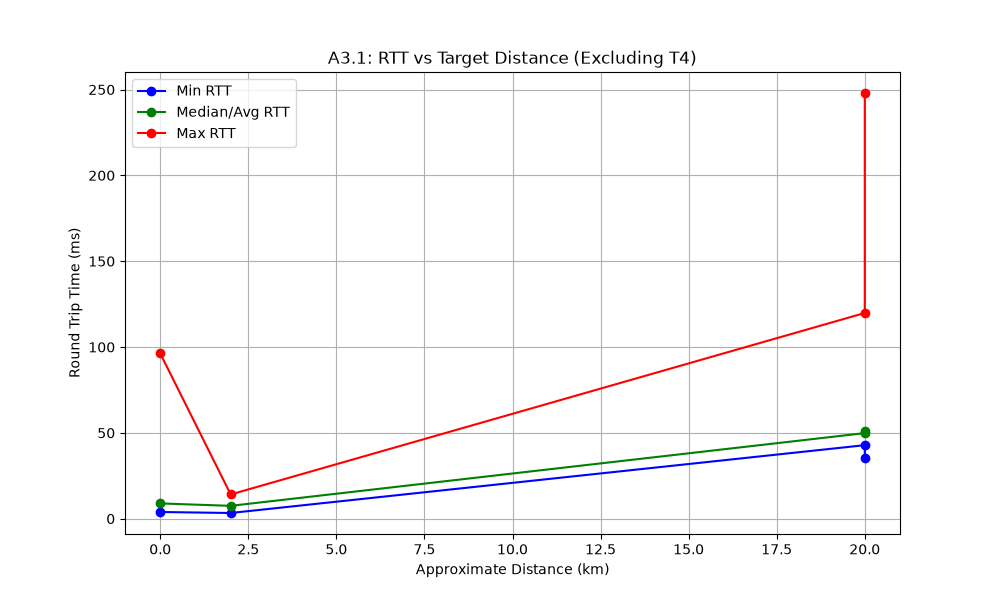
\includegraphics[width=0.75\textwidth]{report/images/a3_1_rtt_vs_distance.png}
    \caption[RTT vs.\ approximate distance]{Minimum, median/average, and maximum RTT against approximate distance for T1, T2, T3, T5 (T4 excluded -- no response).}
    \label{fig:a31plot}
\end{figure}

\textbf{Propagation delay vs.\ measured minimum.} At $2\times10^8$\,m/s, T2's $\sim$2\,km
distance implies a propagation delay of about 0.02\,ms -- negligible next to the measured
3.3\,ms minimum, so for a target this close essentially all of the RTT floor is transmission and
processing delay, not propagation. T5's 12{,}000\,km distance implies a propagation floor of
about 120\,ms round-trip, yet the measured minimum was 35.6\,ms -- well under that floor. The
straightforward reading is that our traffic did not actually travel the full nominal distance:
\texttt{www.mit.edu} is very likely served to us from a CDN edge node much closer than
Massachusetts. An alternative we cannot fully rule out is that the geolocation-based distance
estimate itself is simply wrong (IP geolocation for large anycast/CDN-fronted services is
frequently inaccurate), in which case the ``true'' distance to whatever server actually answered
us is just smaller than 12{,}000\,km rather than the packet having taken an implausible shortcut.
Either way, the number confirms we are not talking to a server in Cambridge, MA.

\textbf{Min-to-max/average gap is queuing delay.} Propagation and transmission delay for a given
path and packet size are effectively fixed, so the spread between the minimum and the
average/maximum RTT for the same target is attributable to queuing delay -- time spent sitting
in router buffers behind other traffic. This is why it shows up as \emph{variation} rather than a
constant offset: queue occupancy depends on how much cross-traffic happens to be competing for
the same link at the moment our packet arrives, which changes probe to probe. T3 shows the
widest such gap (42.8\,ms min vs.\ 119.8\,ms max), consistent with a longer, shared path through
more congested infrastructure than the one-hop path to T1.

\textbf{T1's non-zero RTT.} T1 is one hop away, yet its minimum RTT is 3.9\,ms, not 0. Over
Wi-Fi, this floor is built from MAC-layer overhead we do not see in the ICMP timestamp: CSMA/CA
clear-channel assessment before the medium can be used, the mandatory DIFS/backoff interval,
and (in both directions) the transmission delay of putting the frame on and off the physical
layer, plus whatever small forwarding/processing delay the gateway itself adds. None of this is
propagation delay -- at $<$0.1\,km, propagation is on the order of nanoseconds.

\section{A3.2 -- Making Transmission Delay Visible}
T1 and T3 were pinged at packet sizes 64, 256, 512, 1024, and 1400 bytes (30 packets each); the
minimum RTT at each size was plotted against packet size and fit with a straight line for each
target (Figure~\ref{fig:a32plot}).

\begin{figure}[H]
    \centering
    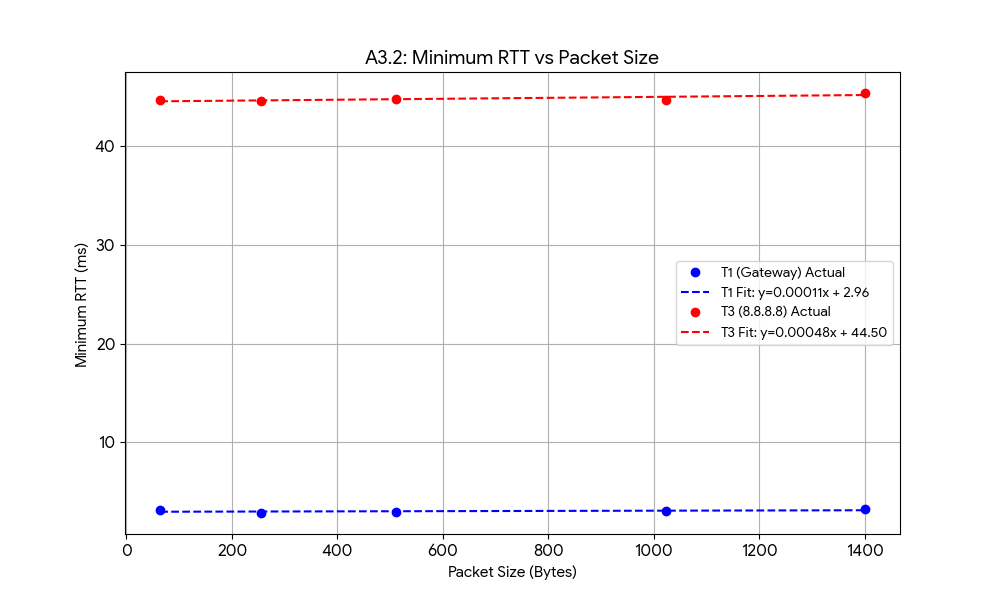
\includegraphics[width=0.75\textwidth]{report/images/a3_2_rtt_vs_packetsize.png}
    \caption[Minimum RTT vs.\ packet size]{Minimum RTT against packet size for T1 and T3, with linear fits.}
    \label{fig:a32plot}
\end{figure}

Fitted lines: T1, $y = 0.00011x + 2.96$; T3, $y = 0.00048x + 44.50$ (RTT in ms, $x$ in bytes).

\textbf{The intercept.} The y-intercept is the extrapolated RTT for a 0-byte payload -- i.e.\
everything that is \emph{not} transmission delay for the payload itself: propagation delay,
router/host processing, and (for T1) Wi-Fi contention overhead. T3's much larger intercept
(44.5\,ms vs.\ 2.96\,ms) reflects the extra propagation and per-hop processing accumulated over
the longer, multi-hop path to 8.8.8.8, versus the single Wi-Fi hop to T1.

\textbf{The slope.} The slope is transmission delay per byte, $L/R$, and since a multi-hop path
uses store-and-forward switching, the effective slope is the \emph{sum} of $1/R_i$ over every
link on the path, not just the first one. T1's slope (0.00011\,ms/byte) is close to flat because
one Wi-Fi hop's link rate is high enough that transmission delay for a payload in this size
range barely moves the RTT. T3's slope (0.00048\,ms/byte) is roughly four times steeper, which is
consistent with the packet crossing several additional links (campus core, egress, upstream)
each contributing their own $L/R_i$ term, rather than transmission delay being determined by a
single bottleneck link. We note that both slopes are small enough, and the underlying ping
resolution coarse enough, that we would not want to over-read the precise ratio between them --
the qualitative story (T3 accumulates more transmission delay across more hops) is what the data
supports; the exact ``4$\times$'' figure is more fragile.

\section{A3.3 -- Watching a Queue Fill}
T3 (8.8.8.8) was pinged continuously for 5 minutes (300 packets) at a quiet hour
(\textcolor{red}{\footnotesize [TODO: exact date]}, 05:30) and again at a busy hour
(\textcolor{red}{\footnotesize [TODO: exact date/time]}). Figure~\ref{fig:a33plot} plots RTT
against sequence number for both.

\begin{figure}[H]
    \centering
    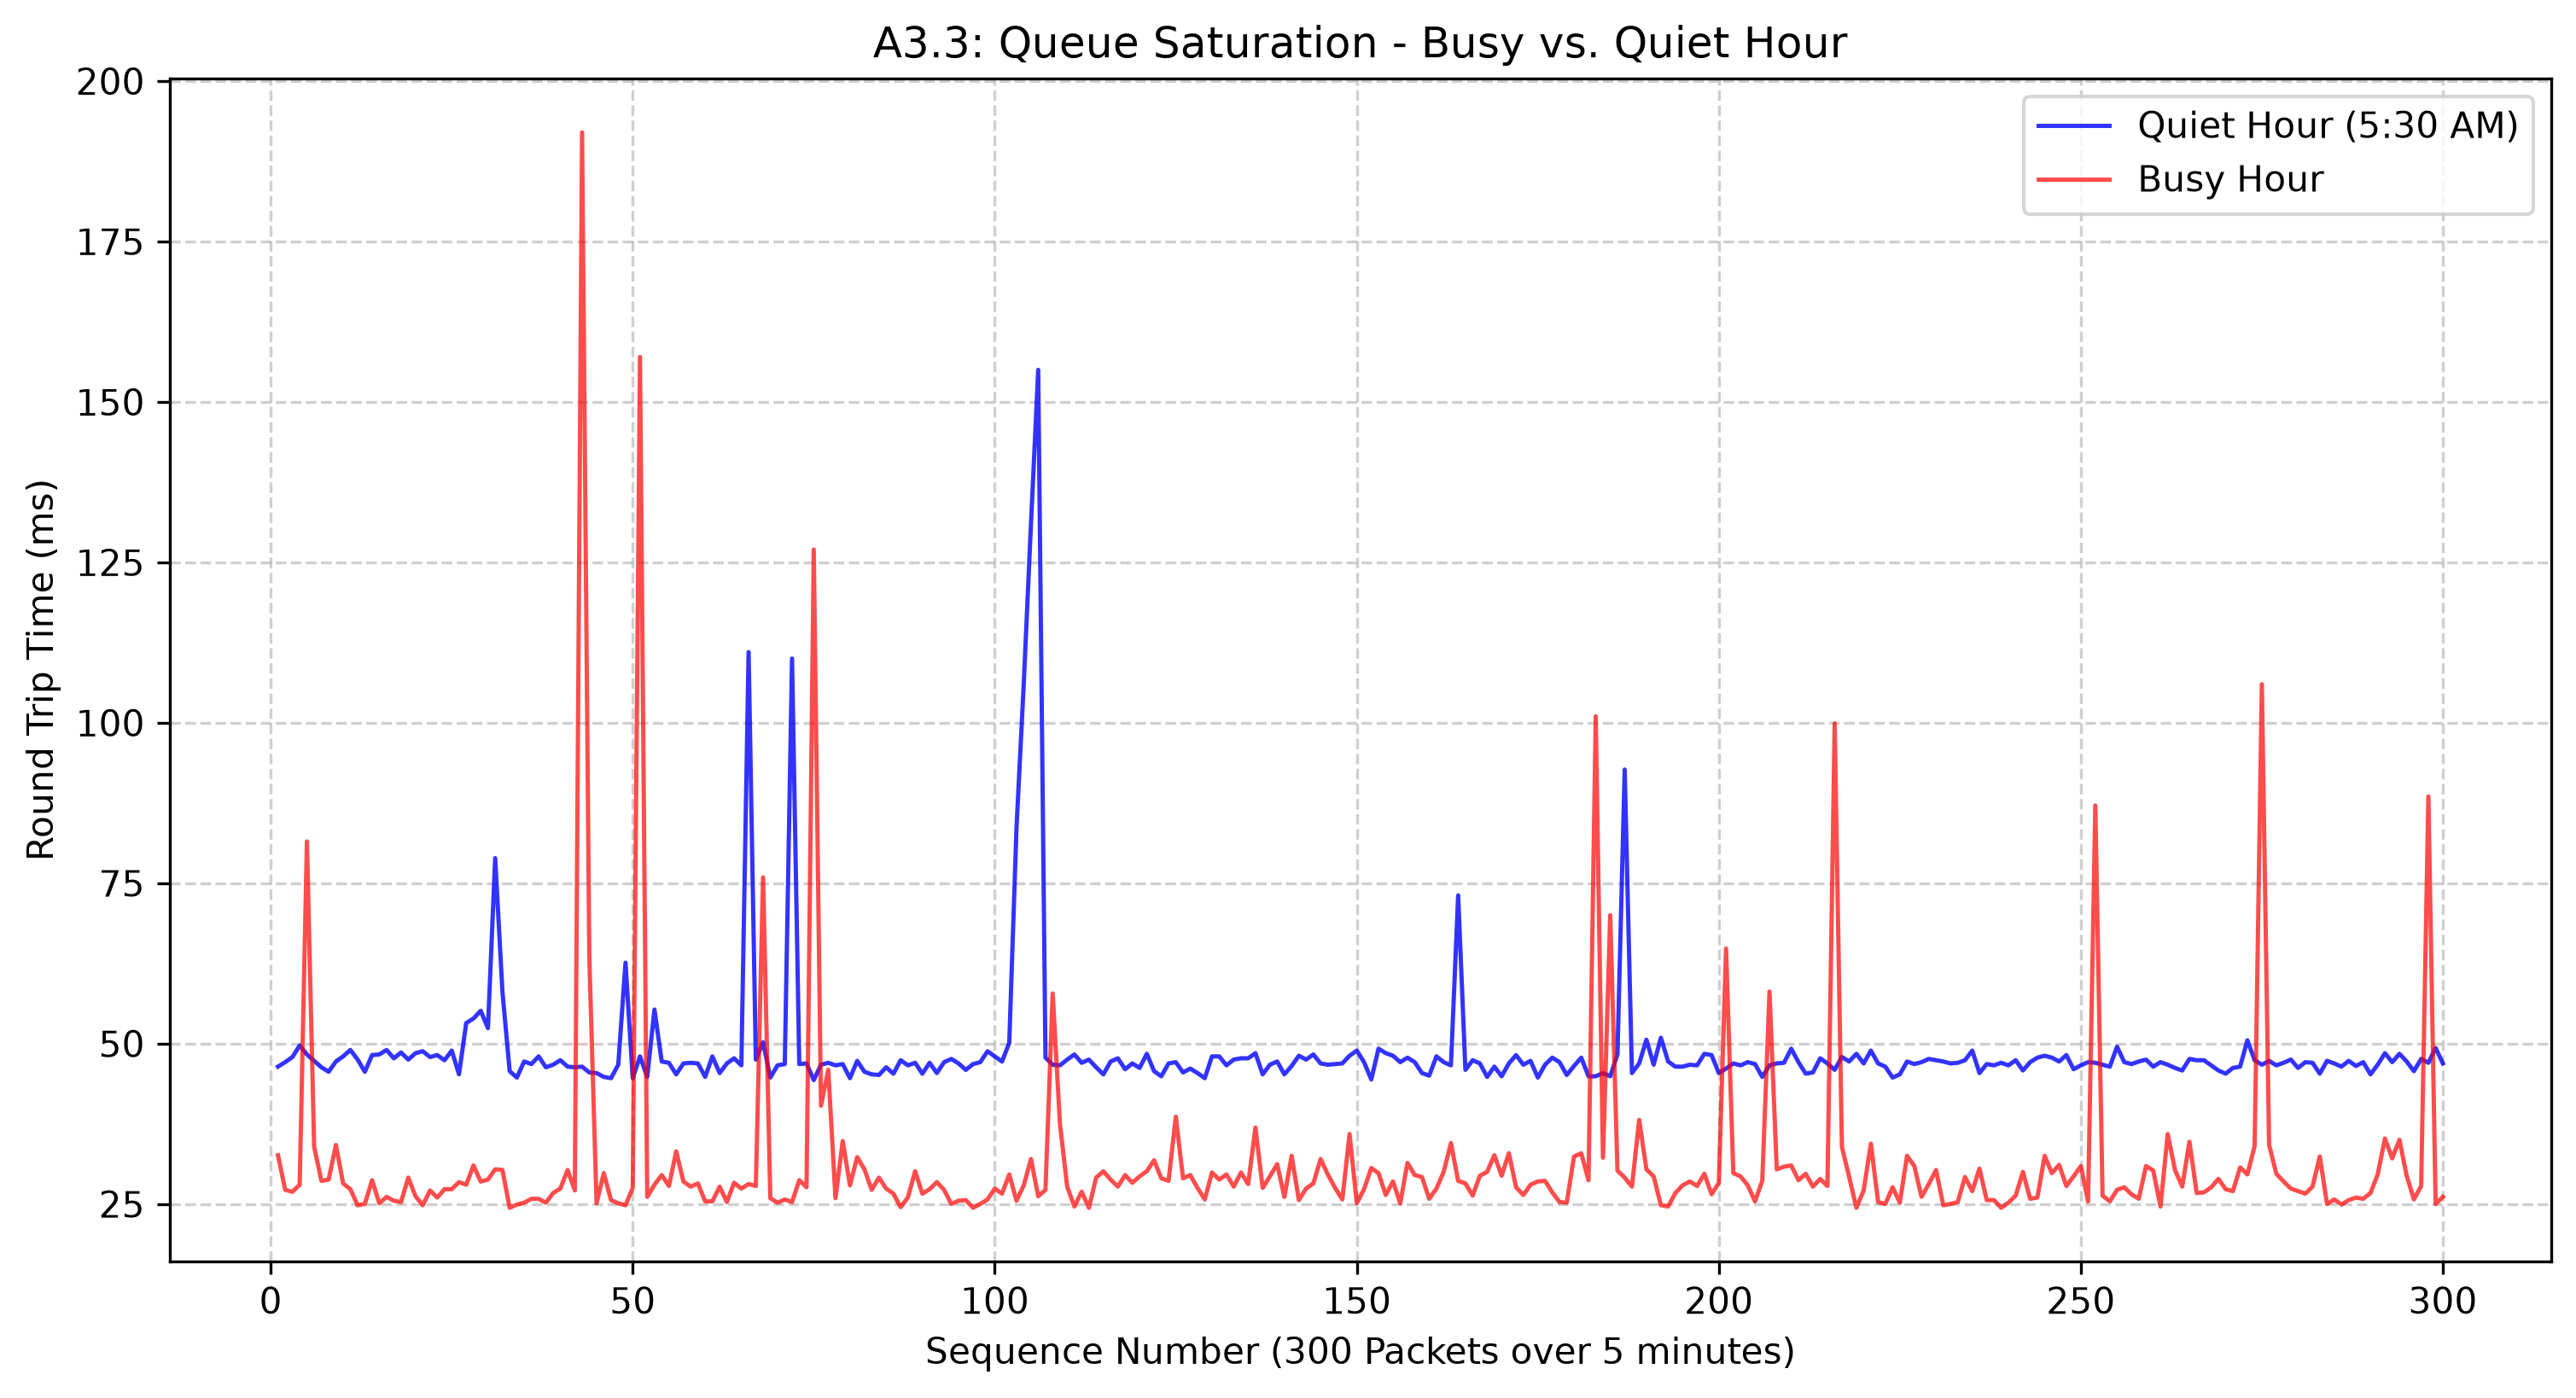
\includegraphics[width=0.85\textwidth]{report/images/A3_3_Queue_Saturation.png}
    \caption[Queue saturation, busy vs.\ quiet hour]{RTT vs.\ packet sequence number, 300 pings to T3, quiet hour (05:30) vs.\ busy hour.}
    \label{fig:a33plot}
\end{figure}

\textbf{Which delay component moved, which didn't.} The spikes in both traces -- and there are
noticeably more of them in the busy-hour trace -- are queuing delay: propagation and
transmission delay for a fixed-size packet on a fixed path do not vary probe-to-probe, so any
variation has to be time spent sitting in a router buffer behind other traffic.

What we did not expect is that the two traces sit on different \emph{baselines}: quiet hour
settles around 48\,ms, busy hour around 27\,ms. Baseline (the floor propagation + transmission +
fixed processing delay would produce with an empty queue) should not depend on time of day, so a
20\,ms shift in the floor itself is not something queuing alone explains. The most likely
account is that the two captures did not use the same path: something changed the route to
8.8.8.8 between the two windows -- most plausibly Google's anycast routing handing us off to a
different, physically closer edge for one of the two captures, though we cannot rule out a
more mundane explanation on our end, such as the device having roamed to a different AP or
uplink between captures. We do not have a way to confirm which, from ping data alone (that would
need a traceroute run in each window, which we did not capture at the time) -- but whichever it
is, it means this pair of captures is confounded for a pure ``same path, different hour'' queuing
comparison, and the baseline shift itself is arguably the more interesting result of the two.

\textbf{What the shape tells us.} Looking past the baseline shift, the two traces do still differ
in shape the way the assignment expects: the quiet-hour trace is flat with only a couple of
isolated spikes (max $\sim$155\,ms), consistent with a queue that is usually empty. The busy-hour
trace is persistently spiky -- frequent, sharp excursions up to $\sim$190\,ms that return to
baseline almost immediately rather than decaying gradually. That shape (sharp in, sharp out,
rather than a sustained elevated floor) reads as bursty cross-traffic -- short bursts that fill a
buffer momentarily and drain quickly once the burst ends -- rather than the queue being
continuously close to full. So while we can't cleanly isolate ``busy hour vs.\ quiet hour on the
same path'', what we can say is that the busy-hour capture, whatever path it took, shows a
network under frequent transient load rather than sustained congestion.
